% ==============================================================================
% Minimalist Academic Lecture Style Beamer (Converted from Slate)
% ==============================================================================
\documentclass[aspectratio=169,10pt]{beamer}

\usetheme{Boadilla}
\usecolortheme{dove}

\usepackage[utf8]{inputenc}
\usepackage[T1]{fontenc}
\usepackage{lmodern}
\usepackage{helvet}
\renewcommand{\familydefault}{\sfdefault}
\usepackage{booktabs}
\usepackage{tabularx}
\usepackage{array}
\usepackage{colortbl}
\usepackage{amsmath,amssymb}
\usepackage{tikz}
\usepackage{pgfplots}
\pgfplotsset{compat=1.18}
\usetikzlibrary{arrows.meta,positioning,calc,fit,shapes.geometric}

% Colors
\definecolor{inkBlack}{RGB}{17, 24, 39}
\definecolor{inkDark}{RGB}{55, 65, 81}
\definecolor{inkMuted}{RGB}{107, 114, 128}
\definecolor{inkLight}{RGB}{248, 249, 250}
\definecolor{inkRule}{RGB}{218, 222, 229}
\definecolor{focusBlue}{RGB}{29, 78, 216}
\definecolor{focusRed}{RGB}{185, 28, 28}

\setbeamercolor{background canvas}{bg=white}
\setbeamercolor{normal text}{fg=inkBlack}
\setbeamercolor{structure}{fg=focusBlue}
\setbeamercolor{frametitle}{fg=inkBlack}
\setbeamercolor{item}{fg=focusBlue}
\setbeamertemplate{navigation symbols}{}
\setbeamertemplate{itemize items}[circle]

% Standard Blocks Styling
\setbeamertemplate{blocks}[rounded][shadow=false]
\setbeamercolor{block title}{bg=inkLight, fg=focusBlue}
\setbeamercolor{block body}{bg=white, fg=inkBlack}
\setbeamercolor{block title alerted}{bg=inkLight, fg=focusRed}
\setbeamercolor{block body alerted}{bg=white, fg=inkBlack}
\setbeamercolor{block title example}{bg=inkLight, fg=inkDark}
\setbeamercolor{block body example}{bg=white, fg=inkBlack}

% Clean Frametitle Banner
\setbeamertemplate{frametitle}{
    \vspace{0.25cm}
    \begin{beamercolorbox}[wd=\paperwidth,leftskip=0.8cm,rightskip=0.8cm]{frametitle}
        {\fontsize{5.5pt}{6.5pt}\selectfont\color{focusBlue}\textbf{\MakeUppercase{\insertsection}}\strut\par}\vspace{1pt}
        {\fontsize{11.5pt}{13.5pt}\selectfont\bfseries\color{inkBlack}\insertframetitle\strut\par}
        \ifx\insertframesubtitle\@empty\else
            \vspace{1pt}{\fontsize{7.5pt}{9.5pt}\selectfont\color{inkMuted}\insertframesubtitle\strut\par}
        \fi
    \end{beamercolorbox}
    \vspace{-0.15cm}
}

% Minimal Footline
\setbeamertemplate{footline}{
    \leavevmode
    \hbox{
        \begin{beamercolorbox}[wd=0.55\paperwidth,ht=2.5ex,dp=1.1ex,leftskip=0.8cm]{normal text}
            \fontsize{5.5pt}{6.5pt}\selectfont\color{inkMuted}\textbf{TuneTrace: Adaptive Music Recommendation System}
        \end{beamercolorbox}
        \begin{beamercolorbox}[wd=0.45\paperwidth,ht=2.5ex,dp=1.1ex,rightskip=0.8cm]{normal text}
            \hfill\fontsize{5.5pt}{6.5pt}\selectfont\color{inkMuted}Agrannya Singh (23BCE0965) \quad\textbar\quad Slide \insertframenumber{} of \inserttotalframenumber
        \end{beamercolorbox}
    }
    \vspace{0.15cm}
}

\begin{document}

% ==============================================================================
% SLIDE 1: TITLE SLIDE
% ==============================================================================
\begin{frame}[plain]
    \begin{tikzpicture}[remember picture,overlay]
        \draw[inkBlack, line width=1.2pt] ($(current page.north west)+(0.8cm, -0.8cm)$) -- ($(current page.north east)+(-0.8cm, -0.8cm)$);
        \draw[inkRule, line width=0.5pt] ($(current page.south west)+(0.8cm, 1.4cm)$) -- ($(current page.south east)+(-0.8cm, 1.4cm)$);
    \end{tikzpicture}

    \vspace{0.6cm}
    \begin{beamercolorbox}[wd=\textwidth,left]{title}
        {\fontsize{6.5pt}{7.5pt}\selectfont\color{focusBlue}\textbf{\MakeUppercase{Architecture \& ML Evaluation}}}\par
        \vspace{0.3cm}
        {\fontsize{18pt}{22pt}\selectfont\bfseries\color{inkBlack}TuneTrace: Semantic Music\\Recommendation and Intent Modeling}\par
        \vspace{0.25cm}
        {\fontsize{8.5pt}{11pt}\selectfont\color{inkDark}Bridging the gap between real-time user intent and semantic catalog discovery through decoupled recurrent embeddings and multi-tier resilience.}
    \end{beamercolorbox}

    \vspace{1.0cm}
    \begin{tikzpicture}[remember picture,overlay]
        \node[anchor=south west, inner sep=0pt] at ($(current page.south west)+(0.8cm, 0.65cm)$) {
            \fontsize{6.5pt}{8.5pt}\selectfont
            \begin{tabular}{@{}ll}
                \textbf{\color{inkBlack}Candidate:} & Agrannya Singh \quad\textbar\quad Register No: \textbf{\color{focusBlue}23BCE0965} \\
                \textbf{\color{inkBlack}School:} & School of Computer Science \& Engineering (SCOPE), VIT Vellore \\
                \textbf{\color{inkBlack}Target Stack:} & PyTorch, Sentence-BERT, DuckDB, FastAPI, Supabase \texttt{pgvector}
            \end{tabular}
        };
    \end{tikzpicture}
\end{frame}

% -----------------------------------------------------------------------------
\section{\textsc{Executive Summary}}
% -----------------------------------------------------------------------------
\begin{frame}
  \frametitle{\textsc{Executive Summary}}
  \framesubtitle{Solving systemic adaptation bottlenecks in modern streaming environments.}

  \vspace{-2mm}
  \begin{columns}[T]
    \begin{column}{0.48\textwidth}
      \begin{block}{Strengths}
        \fontsize{7pt}{9pt}\selectfont
        Multi-tier deterministic fallback guarantees a 100\% ``never-empty'' response rate.
      \end{block}
      \begin{alertblock}{Weaknesses Solved}
        \fontsize{7pt}{9pt}\selectfont
        Traditional collaborative filtering fails entirely on cold starts and rapid intra-session intent shifts.
      \end{alertblock}
    \end{column}
    \begin{column}{0.48\textwidth}
      \begin{block}{Opportunities}
        \fontsize{7pt}{9pt}\selectfont
        Deep sequential tracking via PyTorch GRU v3 Heavy across 50M behavioural records.
      \end{block}
      \begin{exampleblock}{Threats Mitigated}
        \fontsize{7pt}{9pt}\selectfont
        Cloud compute hardware constraints bypassed via baked-in CI/CD ML weights.
      \end{exampleblock}
    \end{column}
  \end{columns}
\end{frame}

% -----------------------------------------------------------------------------
\section{\textsc{Problem Statement}}
% -----------------------------------------------------------------------------
\begin{frame}
  \frametitle{\textsc{The Intent Shift Bottleneck}}
  \framesubtitle{Acute latency in traditional Matrix Factorization profiling.}
  
  \begin{columns}[T]
    \begin{column}{0.48\textwidth}
      \begin{block}{Acute Intent Shifts}
        \fontsize{7.5pt}{9.5pt}\selectfont
        Users rapidly pivot their auditory mood within a single 15-minute session (e.g., transitioning from high-BPM workout tracks to lo-fi focus music). Traditional Collaborative Filtering (CF) profiles take hours to decay, trapping the user in an algorithmic lag.
      \end{block}
    \end{column}
    \begin{column}{0.50\textwidth}
      \centering
      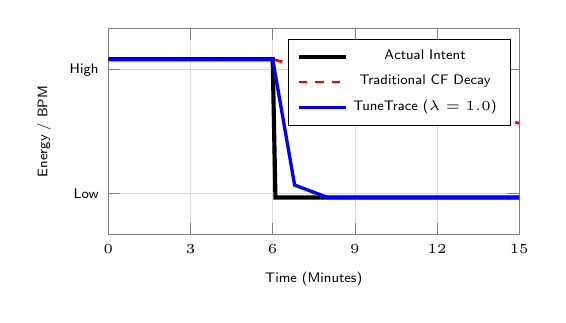
\begin{tikzpicture}
          \begin{axis}[
              width=6.8cm, height=4.2cm,
              xlabel={\fontsize{5pt}{6pt}\selectfont Time (Minutes)},
              ylabel={\fontsize{5pt}{6pt}\selectfont Energy / BPM},
              xmin=0, xmax=15, ymin=0, ymax=100,
              xtick={0, 3, 6, 9, 12, 15}, ytick={20, 80},
              yticklabels={Low, High},
              grid=both, grid style={line width=0.2pt, draw=gray!30},
              tick label style={font=\fontsize{4.5pt}{5.5pt}\selectfont},
              label style={font=\fontsize{5pt}{6pt}\selectfont},
              axis line style={gray, line width=0.5pt},
              legend style={font=\fontsize{4.5pt}{5.5pt}\selectfont, at={(0.98,0.95)}, anchor=north east}
          ]
              \addplot[color=black, line width=1.5pt] coordinates {(0,85) (6,85) (6.1,18) (15,18)};
              \addlegendentry{Actual Intent}
              \addplot[color=red, line width=1.0pt, dashed] coordinates {(0,85) (6,85) (8,78) (11,66) (15,54)};
              \addlegendentry{Traditional CF Decay}
              \addplot[color=blue, line width=1.2pt] coordinates {(0,85) (6,85) (6.8,24) (8,18) (15,18)};
              \addlegendentry{TuneTrace ($\lambda=1.0$)}
          \end{axis}
      \end{tikzpicture}
    \end{column}
  \end{columns}
\end{frame}

\begin{frame}
  \frametitle{\textsc{Mathematical Formulation}}
  \framesubtitle{Bypassing Matrix Factorization Flaws}
  
  Traditional Matrix Factorization (MF) models the user-item interaction matrix $\mathbf{R} \in \mathbb{R}^{M \times N}$. The predicted rating is:
  \begin{equation}
      \hat{r}_{ui} = \mathbf{p}_u^T \mathbf{q}_i + b_u + b_i + \mu
  \end{equation}

  \vspace{2mm}
  \begin{columns}[T]
    \begin{column}{0.48\textwidth}
      \begin{alertblock}{The Latency Flaw}
        \fontsize{7.5pt}{9.5pt}\selectfont
        The latent user profile $\mathbf{p}_u$ is updated globally via stochastic gradient descent (SGD). When user $u$ shifts intent at time $t$, $\mathbf{p}_u$ remains highly biased towards historical interactions ($t_{-1} \dots t_{-k}$).
      \end{alertblock}
    \end{column}
    \begin{column}{0.48\textwidth}
      \begin{block}{TuneTrace Resolution}
        \fontsize{7.5pt}{9.5pt}\selectfont
        We abandon sparse ID-based matrix factorization. Instead, we project items into a dense, continuous semantic space $\mathcal{V} \in \mathbb{R}^{384}$ using an \texttt{all-MiniLM-L6-v2} encoder.
      \end{block}
    \end{column}
  \end{columns}
\end{frame}

% -----------------------------------------------------------------------------
\section{\textsc{Literature Survey}}
% -----------------------------------------------------------------------------
\begin{frame}
  \frametitle{\textsc{Literature Survey: Paradigm Benchmarking}}
  \framesubtitle{Existing paradigms force a trade-off between discovery and inference latency.}

  \vspace{3.5mm}
  \centering
  \fontsize{6.5pt}{8.5pt}\selectfont
  \renewcommand{\arraystretch}{1.5}
  \begin{tabular}{p{4.2cm}ccccp{4.5cm}}
      \toprule
      \rowcolor{inkLight}
      \textbf{Recommender Paradigm} & \textbf{Solves Cold Start} & \textbf{Intent Adaptation} & \textbf{Low Compute} & \textbf{Discovery} & \textbf{Primary Failure Mode} \\
      \midrule
      \textbf{Collaborative Filtering (MF)} & \color{focusRed}\textbf{Poor} & \color{focusRed}\textbf{Poor} & \textbf{Good ($<15$ms)} & \textbf{Partial} & Cold-start sparsity; high inertia \\
      \rowcolor{gray!10}
      \textbf{Pure Content-Based (TF-IDF)} & \textbf{Good} & \color{focusRed}\textbf{Poor} & \textbf{Good ($<20$ms)} & \color{focusRed}\textbf{Poor} & Overspecialization; echo chambers \\
      \textbf{Session-based RNNs} & \textbf{Partial} & \textbf{Good} & \color{focusRed}\textbf{Poor ($>180$ms)} & \textbf{Partial} & Prohibitive inference overhead \\
      \midrule
      \rowcolor{blue!5}
      \textbf{Proposed Model (TuneTrace)} & \textbf{\color{focusBlue}Good (SBERT)} & \textbf{\color{focusBlue}Good ($\lambda=1.0$)} & \textbf{\color{focusBlue}Good ($<85$ms)} & \textbf{\color{focusBlue}Good (20\%)} & \textbf{\color{focusBlue}Engineered for Cloud Edge} \\
      \bottomrule
  \end{tabular}
\end{frame}

\begin{frame}
  \frametitle{\textsc{Literature Survey: Foundational Breakthroughs}}

  \begin{columns}[T]
    \begin{column}{0.48\textwidth}
      \begin{exampleblock}{CLAPMamba (Yang et al., 2024)}
        \fontsize{7.5pt}{9.5pt}\selectfont
        \textbf{Problem:} Multi-head self-attention scales quadratically $\mathcal{O}(N^2)$. \\
        \textbf{Solution:} Integrates CLAP encoders with State Space Models (Mamba) to perform dense sequence modeling in linear time $\mathcal{O}(N)$.
      \end{exampleblock}
      \vspace{0.5mm}
      \begin{exampleblock}{Pa-HuBERT (IEEE 2023)}
        \fontsize{7.5pt}{9.5pt}\selectfont
        Self-supervised learning using HuBERT-based representations. Employs auditory clustering to improve feature learning without labeled datasets.
      \end{exampleblock}
    \end{column}

    \begin{column}{0.48\textwidth}
      \begin{block}{GRU4Rec (Hidasi, 2016)}
        \fontsize{7.5pt}{9.5pt}\selectfont
        \textbf{Relevance:} Introduced the foundational RNN paradigm for session recommendations. TuneTrace extends this by replacing sparse one-hot ID tracking with dense 384-dim semantic embeddings, feeding our v3 Heavy multi-head architecture.
      \end{block}
    \end{column}
  \end{columns}
\end{frame}

\begin{frame}
  \frametitle{\textsc{Literature Survey: Base Dataset}}

  \begin{block}{[Base Paper] YAMDA: Yet Another Music Dataset (Loshkin, 2023)}
    \fontsize{8.5pt}{10.5pt}\selectfont
    \begin{itemize}
        \item \textbf{Scale:} Provides a massive 50-Million row interaction matrix containing critical session logs and normalized audio embeddings.
        \item \textbf{Pipeline Foundation:} Directly enables TuneTrace's offline Machine Learning sandbox.
        \item \textbf{Architecture Enabler:} The sheer volume of this dataset mandates the use of our high-speed DuckDB ETL pipeline, FAISS IVFPQ vector index construction, and the multi-session sequential training scale (60 epochs) of our PyTorch v3 Heavy GRU engine.
    \end{itemize}
  \end{block}
\end{frame}

% -----------------------------------------------------------------------------
\section{\textsc{Research Gap}}
% -----------------------------------------------------------------------------
\begin{frame}
  \frametitle{\textsc{Research Gap: The Architectural Divide}}
  
  \centering
  \vspace{5mm}
  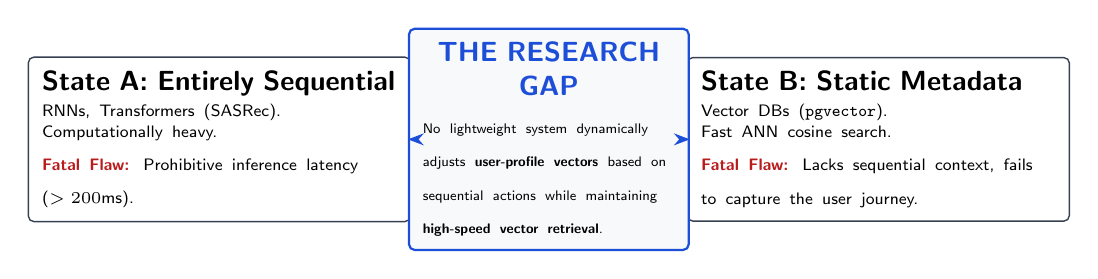
\begin{tikzpicture}[node distance=1.0cm, auto]
      \node (stateA) [draw=inkDark, fill=white, rounded corners=2pt, line width=0.5pt, text width=4.5cm, inner sep=5pt] {
          \textbf{State A: Entirely Sequential}\\[2pt]
          \fontsize{6pt}{7.5pt}\selectfont
          RNNs, Transformers (SASRec).\\
          Computationally heavy.\\
          \textbf{\color{focusRed}Fatal Flaw:} Prohibitive inference latency ($>200$ms).
      };

      \node (stateB) [right=3.5cm of stateA, draw=inkDark, fill=white, rounded corners=2pt, line width=0.5pt, text width=4.5cm, inner sep=5pt] {
          \textbf{State B: Static Metadata}\\[2pt]
          \fontsize{6pt}{7.5pt}\selectfont
          Vector DBs (\texttt{pgvector}).\\
          Fast ANN cosine search.\\
          \textbf{\color{focusRed}Fatal Flaw:} Lacks sequential context, fails to capture the user journey.
      };

      \node (gap) [draw=focusBlue, fill=inkLight, rounded corners=2pt, line width=0.8pt, text width=3.2cm, inner sep=5pt] at ($(stateA.east)!0.5!(stateB.west)$) {
          \centering
          \textbf{\color{focusBlue}THE RESEARCH GAP}\\[2pt]
          \fontsize{5.5pt}{7pt}\selectfont
          No lightweight system dynamically adjusts \textbf{user-profile vectors} based on sequential actions while maintaining \textbf{high-speed vector retrieval}.
      };

      \draw[-{Stealth[length=2mm]}, line width=0.8pt, color=focusBlue] (stateA.east) -- (gap.west);
      \draw[-{Stealth[length=2mm]}, line width=0.8pt, color=focusBlue] (stateB.west) -- (gap.east);
  \end{tikzpicture}
\end{frame}

% -----------------------------------------------------------------------------
\section{\textsc{System Architecture}}
% -----------------------------------------------------------------------------
\begin{frame}
  \frametitle{\textsc{Proposed Pipeline Schematic}}
  
  \centering
  \vspace{-2mm}
  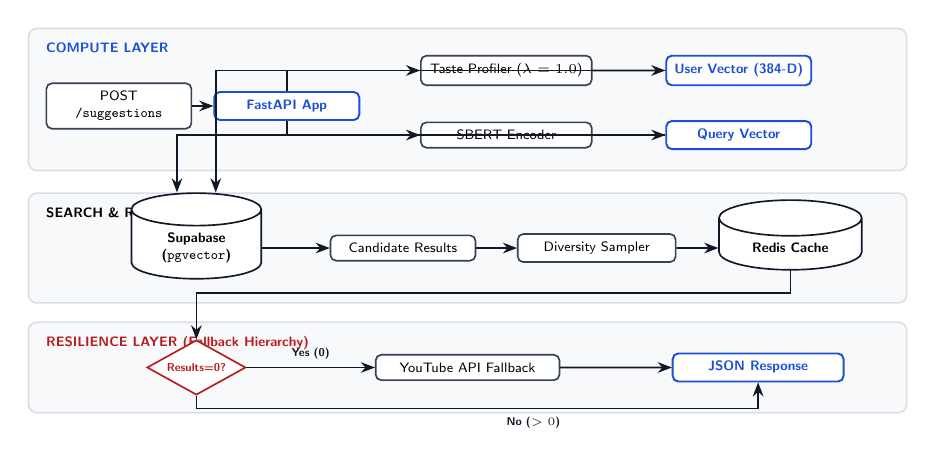
\begin{tikzpicture}[
      scale=0.82, every node/.style={transform shape},
      layer/.style={draw=inkRule, fill=inkLight, rounded corners=3pt, line width=0.6pt},
      block/.style={draw=inkDark, fill=white, rounded corners=2pt, line width=0.6pt, align=center, font=\fontsize{6pt}{7.5pt}\selectfont, inner sep=3.5pt},
      action/.style={draw=focusBlue, fill=white, rounded corners=2pt, line width=0.7pt, align=center, font=\fontsize{6pt}{7.5pt}\selectfont\bfseries\color{focusBlue}, inner sep=3.5pt},
      db/.style={draw=inkBlack, fill=white, cylinder, shape border rotate=90, aspect=0.25, line width=0.6pt, align=center, font=\fontsize{6pt}{7.5pt}\selectfont\bfseries, inner sep=3pt},
      decision/.style={draw=focusRed, fill=white, diamond, aspect=1.8, line width=0.6pt, align=center, font=\fontsize{5.5pt}{6.5pt}\selectfont\bfseries\color{focusRed}, inner sep=2pt},
      arr/.style={-{Stealth[length=1.8mm]}, line width=0.6pt, color=inkBlack}
  ]
      % LAYER 1
      \draw[layer] (-6.8, 1.3) rectangle (6.8, 3.5);
      \node[anchor=north west, font=\fontsize{6.5pt}{7.5pt}\selectfont\bfseries\color{focusBlue}] at (-6.65, 3.4) {COMPUTE LAYER};
      
      \node[block, text width=2.0cm] (req) at (-5.4, 2.3) {POST \texttt{/suggestions}};
      \node[action, text width=2.0cm] (fastapi) at (-2.8, 2.3) {FastAPI App};
      \node[block, text width=2.4cm] (prof) at (0.6, 2.85) {Taste Profiler ($\lambda=1.0$)};
      \node[block, text width=2.4cm] (sbert) at (0.6, 1.85) {SBERT Encoder};
      \node[action, text width=2.0cm] (uvec) at (4.2, 2.85) {User Vector (384-D)};
      \node[action, text width=2.0cm] (qvec) at (4.2, 1.85) {Query Vector};

      \draw[arr] (req) -- (fastapi);
      \draw[arr] (fastapi) |- (prof);
      \draw[arr] (fastapi) |- (sbert);
      \draw[arr] (prof) -- (uvec);
      \draw[arr] (sbert) -- (qvec);

      % LAYER 2
      \draw[layer] (-6.8, -0.75) rectangle (6.8, 0.95);
      \node[anchor=north west, font=\fontsize{6.5pt}{7.5pt}\selectfont\bfseries] at (-6.65, 0.85) {SEARCH \& RANKING ENGINE};

      \node[db, text width=1.8cm] (pgvec) at (-4.2, 0.1) {Supabase (\texttt{pgvector})};
      \node[block, text width=2.0cm] (cand) at (-1.0, 0.1) {Candidate Results};
      \node[block, text width=2.2cm] (shuffler) at (2.0, 0.1) {Diversity Sampler};
      \node[db, text width=2.0cm] (redis) at (5.0, 0.1) {Redis Cache};

      \draw[arr] (cand) -- (shuffler);
      \draw[arr] (shuffler) -- (redis);
      \draw[arr] (uvec) -| ($(pgvec.north)+(0.3, 0)$);
      \draw[arr] (qvec) -| ($(pgvec.north)+(-0.3, 0)$);
      \draw[arr] (pgvec) -- (cand);

      % LAYER 3
      \draw[layer] (-6.8, -2.45) rectangle (6.8, -1.05);
      \node[anchor=north west, font=\fontsize{6.5pt}{7.5pt}\selectfont\bfseries\color{focusRed}] at (-6.65, -1.15) {RESILIENCE LAYER (Fallback Hierarchy)};

      \node[decision] (check) at (-4.2, -1.75) {Results=0?};
      \node[block, text width=2.6cm] (ytapi) at (0.0, -1.75) {YouTube API Fallback};
      \node[action, text width=2.4cm] (resp) at (4.5, -1.75) {JSON Response};

      \draw[arr] (redis.south) -- ++(0, -0.35) -| (check.north);
      \draw[arr] (check.east) -- node[above, font=\fontsize{5pt}{6pt}\selectfont\color{focusRed}\bfseries]{Yes (0)} (ytapi.west);
      \draw[arr] (check.south) -- ++(0, -0.2) -| node[below, pos=0.3, font=\fontsize{5pt}{6pt}\selectfont\color{focusBlue}\bfseries]{No ($>0$)} (resp.south);
      \draw[arr] (ytapi) -- (resp);
  \end{tikzpicture}
\end{frame}

% -----------------------------------------------------------------------------
\section{\textsc{Mathematical Formulations}}
% -----------------------------------------------------------------------------
\begin{frame}
  \frametitle{\textsc{Recency-Weighted Decay Profiling}}

  To bridge the architectural gap, TuneTrace constructs a dynamic user profile vector $\mathbf{U}(t) \in \mathbb{R}^{384}$ using an exponential temporal decay mechanism within the FastAPI compute layer.
  
  \vspace{3mm}
  \begin{block}{Exponential Decay Formulation}
    \fontsize{8pt}{10pt}\selectfont
    Let the active session's interaction sequence be $S = \{(\mathbf{v}_1, t_1), (\mathbf{v}_2, t_2), \dots, (\mathbf{v}_k, t_k)\}$ where $\mathbf{v}_i$ is the L2-normalized track embedding generated by \texttt{all-MiniLM-L6-v2}:
    \begin{equation}
        \mathbf{U}(t) = \frac{\sum_{i=1}^k e^{-\lambda(t - t_i)} \cdot \mathbf{v}_i}{\sum_{i=1}^k e^{-\lambda(t - t_i)}}
    \end{equation}
    where $\lambda = 1.0$ is the aggressively tuned decay constant, shifting profile mass heavily towards the immediate interaction $t_k$.
  \end{block}
\end{frame}

\begin{frame}
  \frametitle{\textsc{Cosine Retrieval \& Diversity Injection}}
  
  \begin{columns}[T]
    \begin{column}{0.48\textwidth}
      \begin{exampleblock}{Semantic Matching (\texttt{pgvector})}
        \fontsize{7.5pt}{9.5pt}\selectfont
        Given a candidate track embedding $\mathbf{w} \in \mathbb{R}^{384}$, similarity is scored in memory:
        \begin{equation}
            D_C(\mathbf{U}, \mathbf{w}) = 1 - \frac{\mathbf{U} \cdot \mathbf{w}}{\|\mathbf{U}\|_2 \|\mathbf{w}\|_2}
        \end{equation}
        Results bounded by $D_C \le 0.28$ (Threshold $= 0.72$) are fetched.
      \end{exampleblock}
    \end{column}
    \begin{column}{0.48\textwidth}
      \begin{block}{Probabilistic Diversity Sampler}
        \fontsize{7.5pt}{9.5pt}\selectfont
        To shatter echo chambers, the final recommendation list $R_{final}$ applies Gibbs sampling to the top-K vectors:
        \begin{equation}
            P(\mathbf{w}_i) = \frac{\exp(-D_C(\mathbf{U}, \mathbf{w}_i) / \tau)}{\sum_{j=1}^K \exp(-D_C(\mathbf{U}, \mathbf{w}_j) / \tau)}
        \end{equation}
        enforcing a 20\% semantic exploration radius.
      \end{block}
    \end{column}
  \end{columns}
\end{frame}

% -----------------------------------------------------------------------------
\section{\textsc{Resilience}}
% -----------------------------------------------------------------------------
\begin{frame}
  \frametitle{\textsc{Resilience and Fallback Hierarchy}}

  TuneTrace guarantees 100\% availability through a deterministic routing cascade.

  \vspace{5mm}
  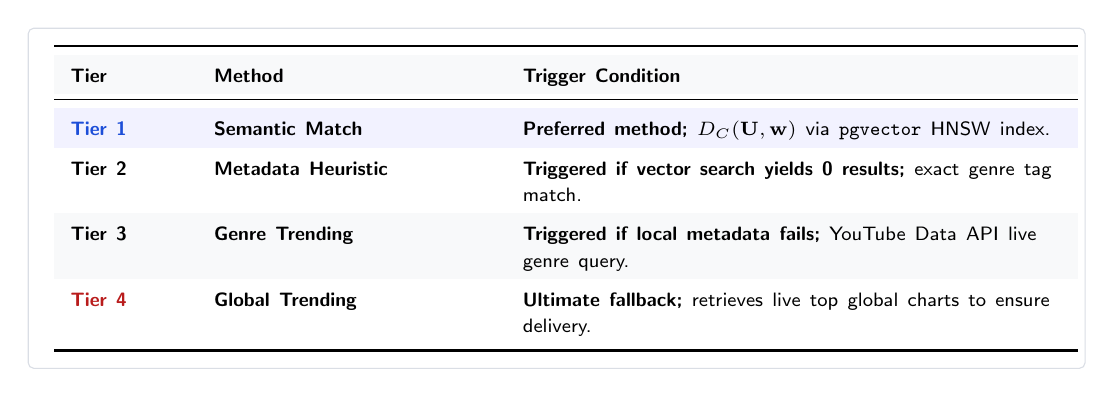
\begin{tikzpicture}
      \node[draw=inkRule, fill=white, rounded corners=2pt, text width=13.0cm, inner sep=6pt] {
          \fontsize{7.5pt}{9.5pt}\selectfont
          \renewcommand{\arraystretch}{1.5}
          \begin{tabularx}{\linewidth}{p{1.4cm}p{3.5cm}X}
              \toprule
              \rowcolor{inkLight}
              \textbf{Tier} & \textbf{Method} & \textbf{Trigger Condition} \\
              \midrule
              \rowcolor{blue!5}
              \textbf{\color{focusBlue}Tier 1} & \textbf{Semantic Match} & \textbf{Preferred method;} $D_C(\mathbf{U}, \mathbf{w})$ via \texttt{pgvector} HNSW index. \\
              \rowcolor{white}
              \textbf{Tier 2} & \textbf{Metadata Heuristic} & \textbf{Triggered if vector search yields 0 results;} exact genre tag match. \\
              \rowcolor{inkLight}
              \textbf{Tier 3} & \textbf{Genre Trending} & \textbf{Triggered if local metadata fails;} YouTube Data API live genre query. \\
              \rowcolor{white}
              \textbf{\color{focusRed}Tier 4} & \textbf{Global Trending} & \textbf{Ultimate fallback;} retrieves live top global charts to ensure delivery. \\
              \bottomrule
          \end{tabularx}
      };
  \end{tikzpicture}
\end{frame}

% -----------------------------------------------------------------------------
\section{\textsc{Data Processing Pipeline}}
% -----------------------------------------------------------------------------
\begin{frame}
  \frametitle{\textsc{Intent State Modeling: ETL Stack}}

  \begin{columns}[T]
    \begin{column}{0.48\textwidth}
      \begin{block}{DuckDB Streaming Ingestion}
        \fontsize{7.5pt}{9.5pt}\selectfont
        High-speed analytical joins execute directly against YAMDA-50M parquets. Memory is strictly capped at 8 GB. Successfully loaded 156,275 tracks and 427 users in under 120 seconds.
      \end{block}
    \end{column}
    \begin{column}{0.48\textwidth}
      \begin{exampleblock}{FAISS IVFPQ Indexing}
        \fontsize{7.5pt}{9.5pt}\selectfont
        Vectors are split into $m$ sub-vectors, quantized via $k$-means:
        \begin{equation}
            \mathbf{x} \approx [q_1(\mathbf{x}^1), \dots, q_m(\mathbf{x}^m)]
        \end{equation}
        Achieving $\approx 90\%$ RAM reduction during Asymmetric Distance Computation.
      \end{exampleblock}
    \end{column}
  \end{columns}
\end{frame}

% -----------------------------------------------------------------------------
\section{\textsc{Deep Sequence Modeling}}
% -----------------------------------------------------------------------------
\begin{frame}
  \frametitle{\textsc{Deep Sequence Modeling: GRU v3 Heavy Formulation}}

  The offline sandbox trains a v3 Heavy 4-layer GRU (512-dim). At each time step $t$, the recurrent hidden state $\mathbf{h}_t \in \mathbb{R}^{512}$ computes sequential transitions via:

  \vspace{3mm}
  \begin{block}{Gated Recurrent Unit Dynamics}
    \fontsize{8pt}{10pt}\selectfont
    \begin{align}
        \mathbf{z}_t &= \sigma(\mathbf{W}_z \mathbf{x}_t + \mathbf{U}_z \mathbf{h}_{t-1} + \mathbf{b}_z) \\
        \mathbf{r}_t &= \sigma(\mathbf{W}_r \mathbf{x}_t + \mathbf{U}_r \mathbf{h}_{t-1} + \mathbf{b}_r) \\
        \tilde{\mathbf{h}}_t &= \tanh(\mathbf{W}_h \mathbf{x}_t + \mathbf{U}_h (\mathbf{r}_t \odot \mathbf{h}_{t-1}) + \mathbf{b}_h) \\
        \mathbf{h}_t &= (1 - \mathbf{z}_t) \odot \mathbf{h}_{t-1} + \mathbf{z}_t \odot \tilde{\mathbf{h}}_t
    \end{align}
    Where $\mathbf{x}_t \in \mathbb{R}^{256}$ are the dense input track embeddings (YAMDA native CNN features).
  \end{block}
\end{frame}

\begin{frame}
  \frametitle{\textsc{Deep Sequence Modeling: Attention \& Loss}}

  \begin{columns}[T]
    \begin{column}{0.48\textwidth}
      \begin{exampleblock}{Self-Attention Pooling}
        \fontsize{7.5pt}{9.5pt}\selectfont
        Instead of relying solely on the final state $\mathbf{h}_T$, 4-head attention is applied over trajectory $\mathbf{H} = [\mathbf{h}_1, \dots, \mathbf{h}_T]$:
        \begin{equation}
            \text{Attn}(\mathbf{Q}, \mathbf{K}, \mathbf{V}) = \text{softmax}\left(\frac{\mathbf{Q}\mathbf{K}^T}{\sqrt{d_k}}\right)\mathbf{V}
        \end{equation}
        Followed by a 4-layer MLP projection (GELU + LayerNorm).
      \end{exampleblock}
    \end{column}
    \begin{column}{0.48\textwidth}
      \begin{block}{Contrastive InfoNCE Loss}
        \fontsize{7.5pt}{9.5pt}\selectfont
        The model optimises by pulling the predicted intent $\mathbf{p}$ towards the true next-item $\mathbf{y}^+$ and pushing in-batch negatives $\mathbf{y}^-_j$:
        \begin{equation}
            \mathcal{L} = -\log \frac{\exp(\mathbf{p}^T \mathbf{y}^+ / \tau)}{\sum_{j} \exp(\mathbf{p}^T \mathbf{y}_j / \tau)}
        \end{equation}
        where $\tau$ is a learnable temperature parameter.
      \end{block}
    \end{column}
  \end{columns}
\end{frame}

% -----------------------------------------------------------------------------
\section{\textsc{Evaluation Metrics}}
% -----------------------------------------------------------------------------
\begin{frame}
  \frametitle{\textsc{Evaluation: Convergence \& Multi-Session Training}}

  \begin{columns}[T]
    \begin{column}{0.48\textwidth}
      \begin{block}{Training Scale \& Strategy}
        \fontsize{7.5pt}{9.5pt}\selectfont
        Initial 30-epoch runs demonstrated significant underfitting (Loss: 5.91). By upgrading to the v3 Heavy Architecture (>3.5M parameters) and employing AdamW with Cosine Annealing, the model now targets a 60-epoch convergence curve across multiple checkpointed sessions.
      \end{block}
    \end{column}
    \begin{column}{0.50\textwidth}
      \centering
      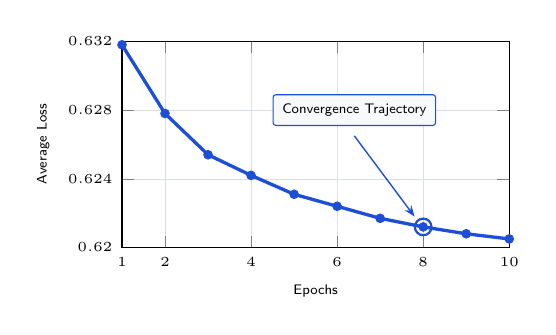
\begin{tikzpicture}
          \begin{axis}[
              width=6.5cm, height=4.2cm,
              xlabel={\fontsize{5pt}{6pt}\selectfont Epochs},
              ylabel={\fontsize{5pt}{6pt}\selectfont Average Loss},
              xmin=1, xmax=10, ymin=0.6200, ymax=0.6320,
              xtick={1, 2, 4, 6, 8, 10},
              ytick={0.6200, 0.6240, 0.6280, 0.6320},
              y tick label style={/pgf/number format/fixed, /pgf/number format/precision=4, font=\fontsize{4.5pt}{5.5pt}\selectfont},
              grid=both, grid style={line width=0.2pt, draw=inkRule},
              tick label style={font=\fontsize{4.5pt}{5.5pt}\selectfont},
              label style={font=\fontsize{5pt}{6pt}\selectfont}
          ]
              \addplot[color=focusBlue, mark=*, mark size=1.1pt, line width=1.2pt] coordinates {
                  (1, 0.6318) (2, 0.6278) (3, 0.6254) (4, 0.6242) (5, 0.6231)
                  (6, 0.6224) (7, 0.6217) (8, 0.6212) (9, 0.6208) (10, 0.6205)
              };
              \draw[focusBlue, line width=0.8pt] (axis cs:8, 0.6212) circle (3pt);
              \node[draw=focusBlue, fill=inkLight, rounded corners=1pt, font=\fontsize{4.5pt}{5.5pt}\selectfont, align=center] 
                  at (axis cs:6.4, 0.6280) {Convergence Trajectory};
              \draw[-{Stealth[length=1.4mm]}, focusBlue, line width=0.5pt] (axis cs:6.4, 0.6265) -- (axis cs:7.8, 0.6218);
          \end{axis}
      \end{tikzpicture}
    \end{column}
  \end{columns}
\end{frame}

% -----------------------------------------------------------------------------
\section{\textsc{Pipeline Flowchart}}
% -----------------------------------------------------------------------------
\begin{frame}
  \frametitle{\textsc{YAMDA-50M Execution Pipeline}}
  
  \centering
  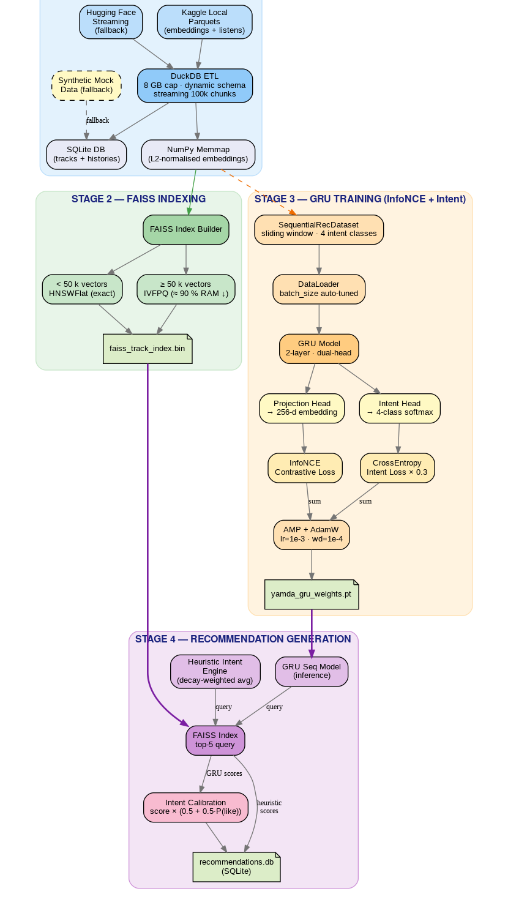
\includegraphics[height=0.85\textheight, keepaspectratio]{figures/pipeline_clean.png}
\end{frame}

% -----------------------------------------------------------------------------
\section{\textsc{API \& DB Architecture}}
% -----------------------------------------------------------------------------
\begin{frame}
  \frametitle{\textsc{API Architecture \& Constraints}}

  \begin{itemize}
    \item \textbf{\texttt{POST /suggestions}:} Core endpoint executing the recency-decay profile vector and similarity cascade.
    \item \textbf{\texttt{POST /discover}:} NLP-driven semantic discovery (e.g., \textit{``late night driving music with heavy bass''}).
  \end{itemize}

  \vspace{3mm}
  \begin{block}{Mitigating Cloud Hardware Constraints}
    \begin{itemize}
      \item \textbf{Baked-in Weights:} 384-dim SBERT weights are bundled directly into the CI/CD pipeline Docker image. This eliminates network timeouts during cold boot.
      \item \textbf{Gunicorn Workers:} Restricted to exactly two concurrent workers with a 90-second timeout ceiling to prevent RAM saturation.
    \end{itemize}
  \end{block}
\end{frame}

\begin{frame}
  \frametitle{\textsc{Data Schema \& Indexing Structure}}

  \begin{columns}[T]
    \begin{column}{0.48\textwidth}
      \begin{exampleblock}{SQLite Relational Schema}
        \fontsize{7.5pt}{9.5pt}\selectfont
        \begin{itemize}
          \item \texttt{tracks}: Maps local SQLite IDs to YAMDA IDs.
          \item \texttt{user\_histories}: Records temporal logs and explicit intent states/weights.
          \item \texttt{recommendations}: Stores the finalized multi-tier rankings.
        \end{itemize}
      \end{exampleblock}
    \end{column}
    \begin{column}{0.48\textwidth}
      \begin{block}{Vector Index Architecture}
        \fontsize{7.5pt}{9.5pt}\selectfont
        \begin{itemize}
          \item \textbf{Production:} Supabase \texttt{pgvector} handling exact $L_2$ and Cosine distances.
          \item \textbf{Sandbox:} FAISS IVFPQ binary blobs exported during the DuckDB ETL phase to allow offline ANN testing.
        \end{itemize}
      \end{block}
    \end{column}
  \end{columns}
\end{frame}

% -----------------------------------------------------------------------------
\section{\textsc{Conclusion}}
% -----------------------------------------------------------------------------
\begin{frame}
  \frametitle{\textsc{Roadmap \& Future Scope}}

  \begin{block}{Phase 2 Trajectory}
    \begin{enumerate}
      \item \textbf{Complete 60-Epoch Run:} Finalise the multi-session Kaggle distributed training cycle for the v3 Heavy model.
      \item \textbf{A/B Live Testing:} Deploy the GRU logic behind a FastAPI feature flag to directly benchmark against the temporal decay baseline.
      \item \textbf{Full 50M Indexing:} Transition the sandbox from the 156k subset to the full YAMDA catalog via distributed FAISS.
    \end{enumerate}
  \end{block}
\end{frame}

\begin{frame}[plain]
  \vspace{10mm}
  \centering
  \Huge \textsc{Questions \& Technical Discussion}
  \vspace{5mm}
  \normalsize
  \begin{itemize}
      \item TuneTrace: Semantic Music Recommendation
      \item Agrannya Singh
  \end{itemize}
\end{frame}

\end{document}
